%------------------------------------------------------------------------- 
\Section{Memory Management}
\label{sec:mmtk}

VMKit uses the Memory Management Tool Kit (MMTK) which is a well-designed and optimized toolkit for writing high performance memory managers. MMTK responsible for memory allocation and reclamation. Here in this section we discuss mainly the composition of MMTK and its functionality as a Garbage Collector (GC) and later we explain how it has been integrated with the VMKit.\\
\subsection{What is MMTK?}
MMTK is an efficient and extensible memory management utility developed using Java ~\cite{mmtk}. Because of the selection of a high level language like java, MMTK has obtained the additional feature of portability which makes it flexible, moreover the clear definition of the interface has enabled it to integrate with different VM with lack of overhead. 
\subsection{Composition of MMTK}
Mechanisms, Policies and Plans are the key compositional elements of the MMTK architecture. The virtual address space is divided typically into 4MB chunks and those are managed with the help of policies defined specifically. In a specific Policy the memory management Mechanism has been implemented. Plans are the highest level of composition which are used to generate Policy objects in order to manage the heap. Figure 3 below illustrates class diagram of the MMTK policies while Figure 4 shows the class diagram of MMTK plans.

\begin{figure}[ht!]
\centering
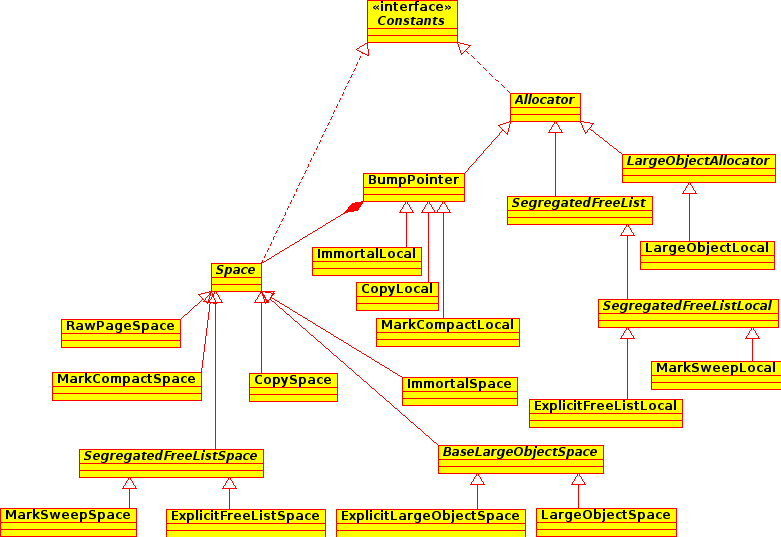
\includegraphics[width=80mm]{Policies.png}
\caption{MMTK policies}
\label{fig:mmtk}
\end{figure}

\begin{figure}[ht!]
\centering
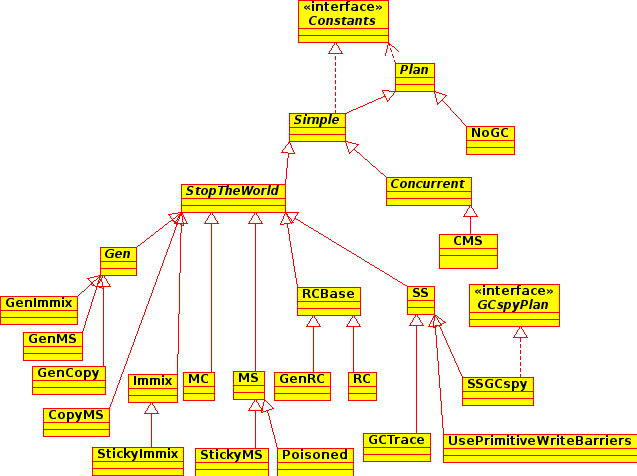
\includegraphics[width=80mm]{Plan.png}
\caption{Class diagram of MMTK plans}
\label{fig:mmtk}
\end{figure}

Following standard allocation and collection mechanisms are implemented by MMTK

\begin{itemize}
 \item \emph{\textbf{Bump Point Allocator}} - When it is requested to allocate memory for a certain object, that object will be appended to the end of the free memory and bump pointer will be incremented to the size of that object.
 \item \emph{\textbf{Free-List Allocator}} - Memory is organized into a segregated free list which keeps a linked list of free memory blocks of a predefined size. When a new object arrives allocation point can be identified from the list with lower search overhead.
 \item \emph{\textbf{Tracing Collector}} - After identifying the live objects by stack maps and write barriers, it reclaim memory by copying them out of the space or by freeing untracked objects.
 \item \emph{\textbf{Reference Counting Collector}}- Keep a count of incoming references for a certain object. If the count become zero, reclaim the memory.
\end{itemize}

Combining the functionalities of above mentioned basic mechanisms, \textbf{Policies} are implemented. Below is the description of few policies.

\begin{enumerate}
 \item Copy Space uses the bump pointer allocation and tracing to trace live objects and copy it to a different location in the memory.
 \item MarkSweep policy uses the free list allocation and tracing collector to track the live objects and reclaim the dead object to the free list.
 \item RefCount policy, here the reference counting collector will claim the non-referenced memory to the free list.
\end{enumerate}

\textbf{Plan} is to instantiate several policies in order to manage the memory. As an instance,
\begin{enumerate}
 \item SemiSpace uses two copies of Copy Space. Memory is divided into two segments, one segment will be allocated while the other is free. When this allocating segment is filled live objects move to the other free segment, and vice versa at next round.
 \item GenCopy, the intuition is to keep one Copy Space for the young objects and transfer the long living objects to an SemiSpace. When the Copy Space is filled then it commences transferring surviving objects freeing the memory, moreover if the old space is filled, entire heap will be collected.  
\end{enumerate}

\subsection{Virtual Machine Interfacing}
Due to the flexibility feature of MMTK it is essential to make the interface of MMTK to the Virtual Machine much clear and well defined. The interface needs to be bidirectional across two entities so that each entity should satisfy specific requirements and features.\\ 
Memory Manager demands requirements such as identification of sources of pointers, low level memory operations such as memcpy, hardware timers, atomic memory operations, I/O etc and virtual machine should cater these requirements as a feature set of the VM. VM pushes the root objects which are the global and local variables on the threads' stacks and registers to MMTK's queue and MMTK enumerates the object pointers and proceed collection.\\
Meanwhile the VM demands requirements such as allocation, write barrier implementation and general statics (Heap size, GC count) from the memory manager. Having this mutual cohesion, VM and MMTK can be integrated. Now in the below sub sections we discuss how VMKit has interfaced with MMTK.\\


\subsection{MMTK integration in VMKit}

According to the discussion in Section 3, the VMKit is a substrate for deveoping Managed Runtime Environments(MRE). Therefore the requirement of the Memory Management module is the independance of other object models or type systems. MMTK has those uniquenss by its design, therefore it is a wise selection for the memory manager in VMKit.\\

Eventhough it is a better selection, below two significant issues have to be rectified in order to integrate MMTK to the VMKit.\\

\begin{enumerate}
 \item Linking MMTK with VMKit, as MMTK is implemented in Java while LLVM and the rest of VMKit are implemented in C++.
 \item Providing MMTK's GCs with exact knowledge of the object location in the heap and the threads execution stacks.
\end{enumerate}


First issue has been resolved with the help of J3 which is a JVM built on top of VMKit. According to the figure 3, J3 is used in order to load and compile MMTK during the compilation of VMKit. At this point the J3 is executed with a lightweight memory manager and rest of the VMKit uses the LLVM ahead of time compiler to generate the LLVM bytecode of MMTK. After generating the LLVM bytecodes those are not dependent on other runtime environments, now the VMKit loads and dynamically compiles them before launch a high level MRE.\\

\begin{figure}[ht!]
\centering
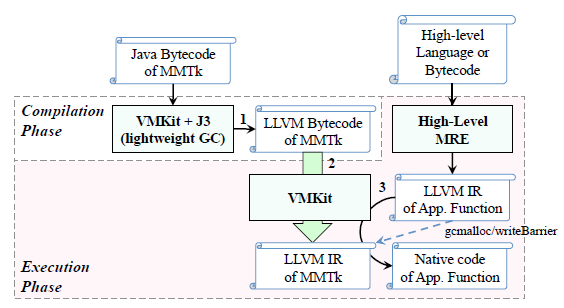
\includegraphics[width=80mm]{vmkitmmtk.png}
\caption{ Integration of MMTk in VMKit. Solid arrows are compilations or transformations. Dashed arrows are invocations. The big solid arrow is the initialisation phase of VMKit}
\label{fig:mmtk}
\end{figure}

As a solution for the second issue, the MRE has to provide the functions for the GC to accurately scan the heap. These functions are highly dependent on the execution stack layouts and the object model of the MRE and those are indicated in figure 2.(See the box GC related functions.) \\

Moreover, the GC does not have the knowledge of the object lay out as well as the global roots of object graph which depicts the global variables, constant objects, classes, fields etc. Therefore the MRE needs to provide those required details with the help of LLVM built in intrinsic. For instance , the intrinsic called gcroot which is provided by LLVM takes an abstract register as an argument which contains a reference and generates the stack map (Stack map indicates where the root objects are located in a frame). Furthermore MRE provides functionality for the MMTK to trace the objects so that GC can traverse the directly reachable sub objects of each object.\\

Once the high level MRE is loaded the mutual interactions between the interfaces of VM and MMTK takes care of the memory management of the system as a whole.

\subsection{Allocation}
MMTK provides two methods for allocating memory. One is the unsynchronized thread local allocation which is used by each policy by means of thread local classes while the other one is slower synchronized slow path allocation which is related to the global memory abstraction shared by multiple mutator threads. The idea here is allocating memory from thread local buffer and when that memory is fully allocated additional memory will be allocated from the global space.\\

For instance below code segment is a simplified version of allocation of a segregated free list implementation which initially checks the thread local buffer and if unsuccessful move for the slow allocation method which will ultimately uses a global policy.\\

\begin{figure}[ht!]
\centering
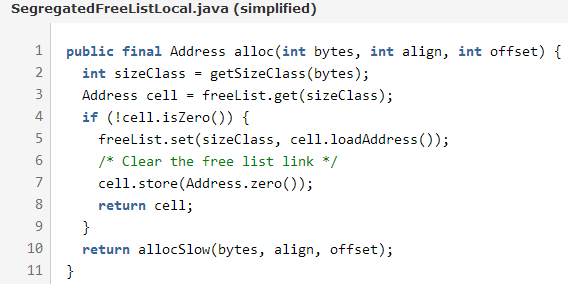
\includegraphics[width=80mm]{code_1.png}
\caption{Segregated free list implementation}
\label{fig:mmtk}
\end{figure}

Eventually all the policies will acquire virtual memory by calling the acquire method of the Space global object. Below code segment shows a simplified view of that method.\\

\begin{figure}[ht!]
\centering
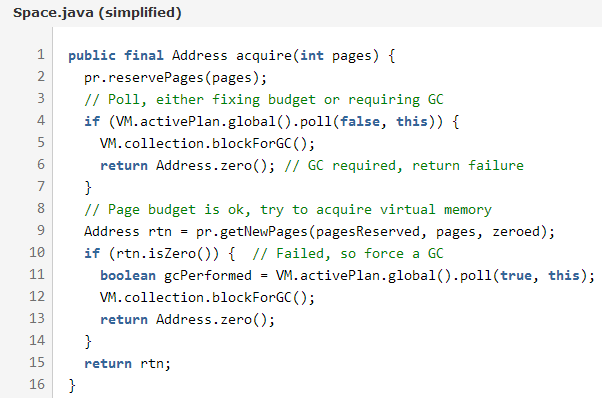
\includegraphics[width=80mm]{code_2.png}
\caption{Simplified view of the space global object implementation}
\label{fig:mmtk}
\end{figure}

Here it contacts the plan which know the policy objects generated for memory management to check whether the heap is fully allocated, if so wait for the GC to collect and free the memory, otherwise return the requested page's memory address.\\

\subsection{Collection}
Memory reclamation can be scheduled in two ways as stop the world garbage collection and parallel garbage collection. In the former schedule, mutator (appliation) are executed until the memory is exhausted and then the mutator threads are suspended untill the garbage collection is completed. In the latter schedule collector threads are allowed to execute parallel with the mutator threads.\\

As mentioned in the previous memory allocation related details, in each attempt to access fresh virtual memory force to initiate a garbage collection. Every garbage collection is a flow of multiple steps.  